\subsection{Introduction to Time Series}
Models are not always \textit{independent of the order} of the training data. Many real life measuring and data recording processes result in data sets that are \textit{serially correlated}. For example \textit{machine monitoring, stock, environmental observations or federal statistics.} These kind of data is called \textit{time series data}. Usually there are several goals that one wants to achieve in time series data.
\begin{itemize}
	\item \textbf{Descriptive Analysis}
	\item \textbf{Modelling and Interpretation}
	\item \textbf{Decomposition}
	\item \textbf{Predection}
	\item \textbf{Regression}
\end{itemize}
\subsubsection{Time Series with \color{blue}R}
{
\RTheory
{	All data in {\color{blue}R} are stored in objects, which provide a range of methods. The class of an object can be found using the {\color{blue}class} function. For example, we have already encountered the {\color{blue}data.frame} class. It has a series of methods, such as {\color{blue}names} or {\color{blue}nrow}: \vfill
(The data set iris contains 50 samples of three types of Iris flowers, measured along four variables.)}
{sections/TimeSeriesAnalysis/IntroductionToTimeSeries/RCode/timeSeries.R}
\paragraph{The {\color{blue}ts} Class}
{\RTheory
{\textbf{Basic properties:}\vfill
	The AirPassengers-data is a built in set of class {\color{blue}ts}. Most important methods for {\color{blue}ts} class are:\vfill 
\begin{enumerate}
\item  {\color{blue}start()} returns the start time of the series.
\item  {\color{blue}end()} returns the end time of the series.
\item  {\color{blue}frequency()} returns the number of samples per unit time.
\item  {\color{blue}plot()} displays the time series as a function over the time axis. {\color{blue}plot} function calls {\color{blue}plot.ts} which is tailored for time series. {\color{blue}plot.ts} joins discrete time points automatically with lines.  See Figure AirPassengers. 
\end{enumerate}}
{sections/TimeSeriesAnalysis/IntroductionToTimeSeries/RCode/tsClassBasic.R}
\begin{figure}[H]\centering
	\begin{minipage}[c]{0.5\textwidth}
	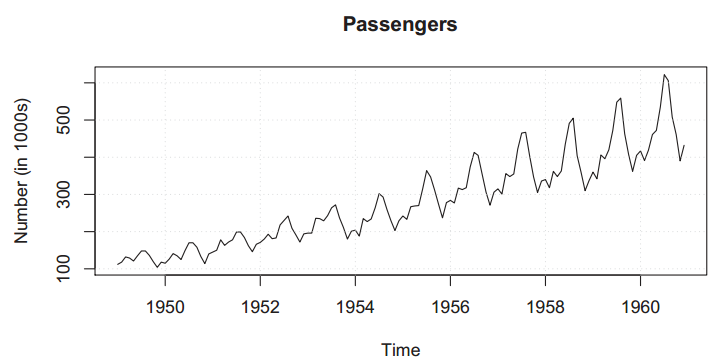
\includegraphics[width=1\linewidth]{images/tsAirPassengers.png}
		\caption{AirPassengers}
	\end{minipage}\hfill
	\begin{minipage}[c]{0.5\textwidth}
	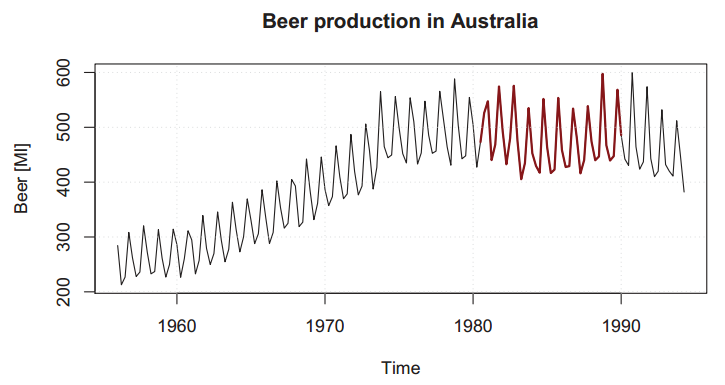
\includegraphics[width=1\linewidth]{images/tsSeasBehav.png}
	\subcaption{Subset of a Time Series (seasonal behaviour)}
	\end{minipage}\hfill
\end{figure}
\RTheory
{
\textbf{Defining a {\color{blue}ts} class}\vfill
If data is not in a time series form we can make a {\color{blue}ts} object by using the {\color{blue}ts}  function. This is not necessary for AirPassengers, therefore the example AustralianBeer is used.
\begin{enumerate}
	\item  {\color{blue}summary()} gives the five-number summary as well as the mean of the time series.This function shows the minimum, the first quartile, the median, the second quartile and the maximum of the time series. This is called the \textit{five-number-summary} of a data set. Additionally the mean is also computed.
	\item  {\color{blue}window()} returns a subset of the time series defined by a start and an end time.
\end{enumerate}
}
{sections/TimeSeriesAnalysis/IntroductionToTimeSeries/RCode/tsClassDefining.R}
\RTheory
{
\textbf{Multivariate Time Series}\vfill
A few important ideas and concepts related to multivariate time series data illustrated with the following example:\vfill
\hfill
\break
The quaterly supply of electricity in Australia compared to the quaterly beer production see Figure \ref{Fig:BeerVsElectricity}.\vfill
The plots show increasing trends in production for both goods, partly
due to the rising population in Australia from about 10 million to about 18 million over the same period. But notice that electricity production has risen by a factor of 7 during which the population has not quite doubled. \vfill
\hfill
\break
There are many functions in {\color{blue}R} for
handling more than one series, including {\color{blue}ts.intersect} to obtain the intersection
of two series that overlap in time. There are some \textbf{pitfalls} shown with AirPassenger and electricity in Figure \ref{Fig:APVsElectricity}. \vfill
\hfill
\break
The two series are correlated but there is of course \textbf{no causal dependence} of the two series. They are confounded by seasonal effects.
\vfill
\hfill
\break
\textbf{Non-equdistant time series} are \textbf{not covered} by the {\color{blue}ts} class. There are further packages:
\begin{itemize}
	\item \textbf{{\color{blue}zoo-}package}:It provides methods for regular and irregular spaced times series as well as arbitrary date formats.
	\item \textbf{{\color{blue}xts-}package}: It is an extension of the {\color{blue}zoo-}package which allows for further customzation.
\end{itemize}
}
{sections/TimeSeriesAnalysis/IntroductionToTimeSeries/RCode/tsMultivariateTimeSeries.R}
\begin{figure}[H]\centering
		\begin{minipage}[t]{.5\textwidth}
		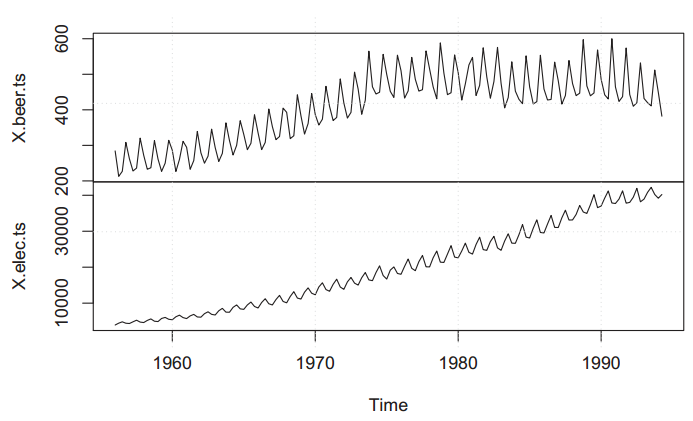
\includegraphics[width=1\linewidth]{images/tsBeerVsElec.png}
		\subcaption{Beer and electricity production in Australia}
		\label{Fig:BeerVsElectricity}
	\end{minipage}\hfill
	\begin{minipage}[t]{.5\textwidth}
		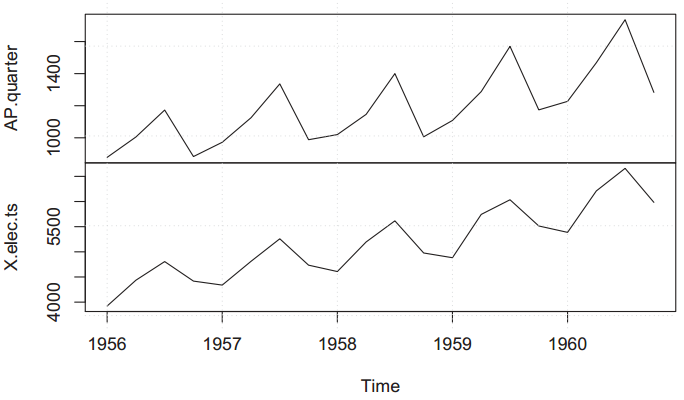
\includegraphics[width=1\linewidth]{images/tsAPVsElec.png}
		\subcaption{Air Passenger bookings and electricity production}
		\label{Fig:APVsElectricity}
	\end{minipage}
\end{figure}

}
\subsubsection{Basic transformation, visualization and decomposition of time series}
{\paragraph{Data transformation}
	In many situtions it is desirable or necessary to transform a time series before the application of models and predictions. Many methods require
	\begin{itemize}
		\item \textbf{Gaussian} or \textbf{symmetric} distribution of the data.
		\item A \textbf{linear} trend relationship between time and data.
		\item A \textbf{constant variance} across time.
	\end{itemize}
\RTheory
{\textbf{Box-Cox-transformation}\vfill
For highly skewed or heteroskedastic data - data whose variance is not constant across time - it is often better to use not the original series $\{x_1, x_2, ...\}$ but a transformed series $\{g(x_1), g(x_2),...\}$. The Box-Cox-transformation is well suited for correcting skewness and variance.
\vfill
\hfill
\break
For a times series $\{x_1, x_2, . . . \}$ with positive values the Box-Cox transformations
are defined as
$$ g(x)=\begin{cases}
\frac{x^{\lambda}-1}{\lambda} &\lambda \neq 0\\
log(x) &\lambda = 0\\
\end{cases}$$
As in Figure \ref{Fig:boxCox} to see the original data exhibits clear seasonal effects and an upward trend.The intensity of
the seasonal influence, i.e. the variance over time, is also increasing. The parameter $\lambda$ = 0, i.e. the log-transform of the data, yields a stabilized image: a
seemingly linear trend with homogeneus seasonal effects.
}
{sections/TimeSeriesAnalysis/IntroductionToTimeSeries/RCode/boxCoxTransformation.R}
\begin{figure}[H]\centering
	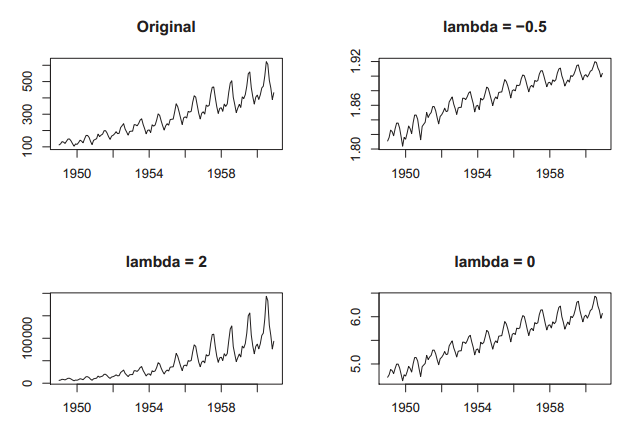
\includegraphics[width=0.7\linewidth]{images/boxCox.png}
	\caption{Box-Cox-transformation for different values of $\lambda$}
	\label{Fig:boxCox}
\end{figure}
\RTheory
{\textbf{Time-shift transformation}\vfill
	Sometimes it is necessary to transform the time-axis as well. The most simple form version of time transforms is shifting.
	\vfill
	\hfill
	\break
	Let $\{x_1, x_2, . . . \}$ be a time series.
	\begin{enumerate}
	\item The time-shift by a \textit{lag} of $k \in \mathbb{Z}$ is defined by
	$$g(x_i)=x_{i-k} $$ 
	\item For the particular case where $k=1$ the time-shift is called \textit{backshift}
	$$ B(x_i)=x_{i-1}$$ 
	\end{enumerate}
	In other words, applying a time-shift to a time series amounts to go back $k$ steps (if $k>0$) or go ahead $-k$ steps (if $k<0$) in the series.
	\vfill
	\hfill
	\break
	In {\color{blue}R} the function {\color{blue}lag} is used to apply a time shift for various values of $k$.
\vfill
\hfill
\break
The back-shift operator is applied if \textit{differences} of times series are computed, since $x_i - x_{i-1}=x_i-B(x_i)$. In particular, differencing is often combined with Box-Cox
transformations. For example in the \textit{log-returns} of a (financial) time series are defined as
$$ y_i = log(x_i)-log(x_{i-1}) = log\bigg(\frac{x_i}{x_{i-1}}\bigg)$$

}
{sections/TimeSeriesAnalysis/IntroductionToTimeSeries/RCode/timeShiftTransformation.R}
\begin{figure}[H]\centering
	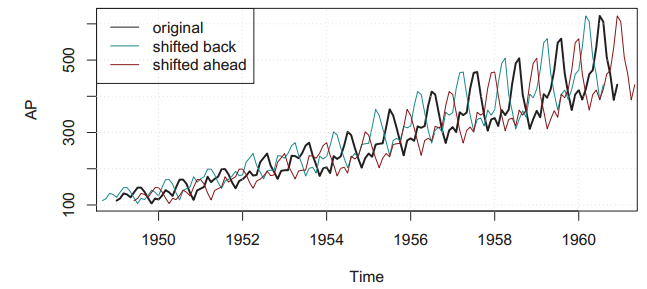
\includegraphics[width=0.7\linewidth]{images/timeShiftTrans.png}
	\caption{Time-shift transformation}
	\label{Fig:timeShiftTrans}
\end{figure}
\paragraph{Visualizations}
\RTheory
{\textbf{Visualization Example}\vfill
We have hourly measurements of several sensors, where we now focus on the air temperature. The time series is defined with a basic units of days starting at day 1 and frequency 24. The {\color{blue}end()}-command shows that the time series lasts 396 days and 8 hours, or in other words, has 9512 data points. The plot in Figure \ref{Fig:tsAirTempFull} shows the complete time series. The {\color{blue}ylim} option limits the temperature axis to nonnegative values.
\vfill
\hfill
\break
We focus on a period of 20 days to analyse the temperature behaviour in more detail. Figure \ref{Fig:tsAirTempDetail} shows the data.
\vfill
\hfill
\break
Figure \ref{Fig:tsBoxPlot} shows how data aggregation can be visualized with the {\color{blue}boxplot}-command. We are going to generate a boxplot for each full hour in one figure. To this end the {\color{blue}cycle()} function is very convenient: it returns for a given time series the positions in the cycle of each observation. In our example, a cycle is one day consisting of 24 hours. This means, that the first entry in the time series is at cycle position 18, i.e. measuredat 6 p.m. and that the 875-th measurement is at cycle position 4, which corresponds to 4 a.m. The subset of observations that share a common cycle are called cycle-subseries and will be used later for time series decomposition.
\vfill
\hfill
\break
A useful graphical approach for visually inspecting correlations of consecutive observations are \textit{lagged scatterplots}. They amount to produce scatterplots of the original time series values against a time-shiftet version, i.e. plotting the data pairs $(x_i, x_{i-k})$.
This can be done in {\color{blue}R} by the {\color{blue}lag.plot} command. Figure \ref{Fig:tsLagPlot} shows that the scatterplot with lag 1 shows a linear pattern which indicates a correlation. A lag of 10 hours results in a unspecific scatter plot.
}
{sections/TimeSeriesAnalysis/IntroductionToTimeSeries/RCode/tsVisualization.R}
\begin{figure}[H]\centering
	\begin{minipage}[c]{0.42\textwidth}
		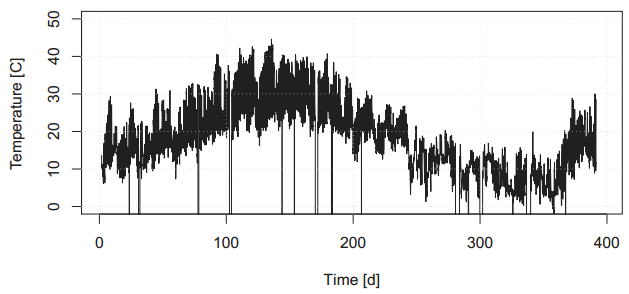
\includegraphics[width=1\linewidth]{images/tsAirTempFull.png}
		\subcaption{Air temperature measurement: 9512 points}
		\label{Fig:tsAirTempFull}
	\end{minipage}
	\begin{minipage}[c]{0.42\textwidth}
		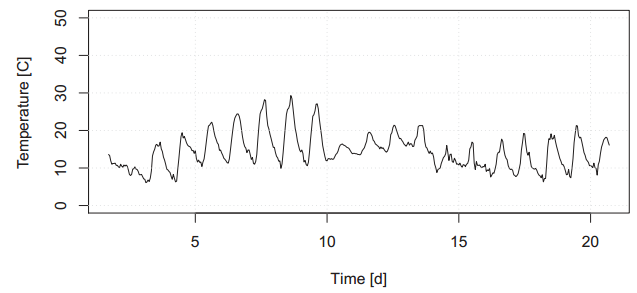
\includegraphics[width=1\linewidth]{images/tsAirTempDetail.png}
		\subcaption{Air temperature measurement: 480 points}
		\label{Fig:tsAirTempDetail}
	\end{minipage}
	\begin{minipage}[t]{.42\textwidth}
		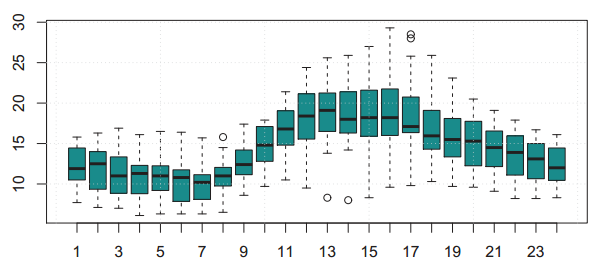
\includegraphics[width=1\linewidth]{images/tsBoxPlot.png}
		\subcaption{Air temperature: Boxplot}
		\label{Fig:tsBoxPlot}
	\end{minipage}
	\begin{minipage}[t]{.42\textwidth}
		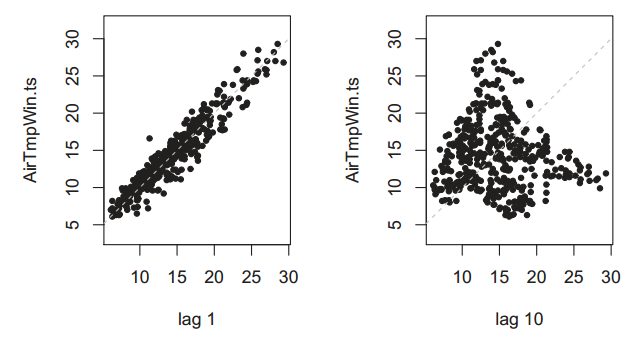
\includegraphics[width=1\linewidth]{images/tsLagPlot.png}
		\subcaption{lag.plot}
		\label{Fig:tsLagPlot}
	\end{minipage}
\caption{Visualization}
\end{figure}
\paragraph{Decomposition of time series}
\begin{figure}[H]\centering
	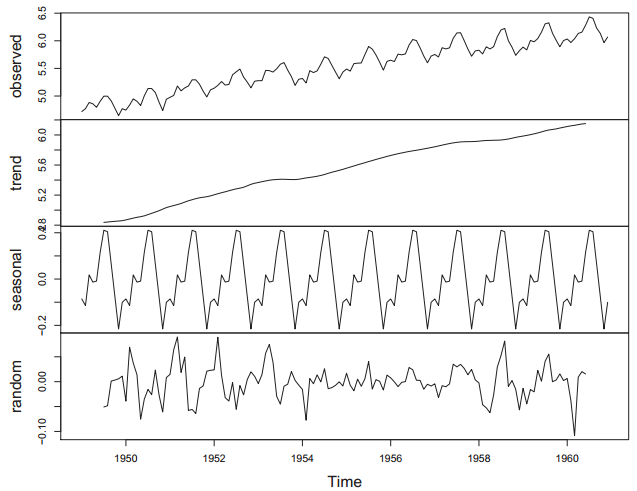
\includegraphics[width=0.7\linewidth]{images/tsDecomposition.png}
	\caption{Decomposition of additive time series}
	\label{Fig:tsDecomposition}
\end{figure}
\RTheory
{\textbf{Moving Average}\vfill
A simple additive decomposition model is given by
$$x_k = m_k + s_k + z_k $$
where at time index $k$, $x_k$ is the observed series, $m_k$ is the trend,  $s_k$ is the seasonal effect, and $z_k$ is an error term that is, in general, a sequence of \textit{correlated} random variables with mean zero.
\vfill
\hfill
\break
In the AirPassenger data the seasonal effects may increase as the trend increase. Thus a multiplicative model is more convenient
$$ x_k = m_k \cdot s_k + y_k $$
If the noise is multiplicative as well, the logarithm of $x_k$ is a linear model again
$$log(x_k) = log(m_k) + log(s_k) + log(y_k) $$
A simple method for estimating $m_k$ and $s_k$ is by means of the moving average filter. Assume that $\{x_1,x_2,...,x_k \}$ is a time series and that $p \in \mathbf{N}$. The \textit{moving averaage filter} of length $p$ is defined as follows
\begin{itemize}
	\item  If $p$ is odd, then $p=2l + 1$ and the filtered sequence is defined by
	$$ g(x_i)= \frac{1}{p}(x_{i-l}+...+x_i+...+x_{i+l})$$ 
	\item  If $p$ is even, then $p=2l$ and the filtered sequence is defined by
	$$ g(x_i)= \frac{1}{p}(\frac{1}{2}x_{i-l}+x_{i-l+1}+...+x_i+...+{i+l-1}+\frac{1}{2}x_{i+l})$$ 
\end{itemize}
The value $p$ is referred to as \textit{window width}. 
\vfill
\hfill
\break
Estimate seasonal additive effect: $\hat{s_k}={x_k}-\hat{m_k}$
\vfill
\hfill
\break
Remainder: $\hat{r_i}=x_i-\hat{m_i}-\hat{s_i}$
\vfill
\hfill
\break
To diminsh the non-random parts the steps are repeated with the logarithm model. AirPassenger amounts to a multiplicative model.
}
{sections/TimeSeriesAnalysis/IntroductionToTimeSeries/RCode/tsDecomposition.R}
\RTheory
{
\textbf{Seasonal Decomposition of Time Series by Loss (STL)}\vfill
The decomposition method above is seldomly used because of several reasons. Hence the {\color{blue}stl()} function is used. Two mandatory parameters have to be passed to it:
\begin{enumerate}
	\item {\color{blue}x} he time series to be decomposed
	\item {\color{blue}s.window} he loess window size for the seasonality component. The larger the value the slower the change of seasonality in the data set over time.
\end{enumerate}
}
{sections/TimeSeriesAnalysis/IntroductionToTimeSeries/RCode/tsSTL.R}
\begin{figure}[H]\centering
	\begin{minipage}[c]{0.5\textwidth}
	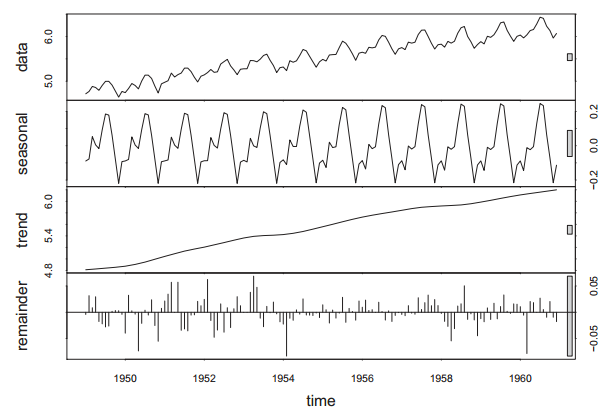
\includegraphics[width=1\linewidth]{images/tsSTL.png}
	\subcaption{STL decomposition of the log of AirPassengers data}
	\label{Fig:tsSTL}
\end{minipage}\hfill
\begin{minipage}[c]{0.5\textwidth}
	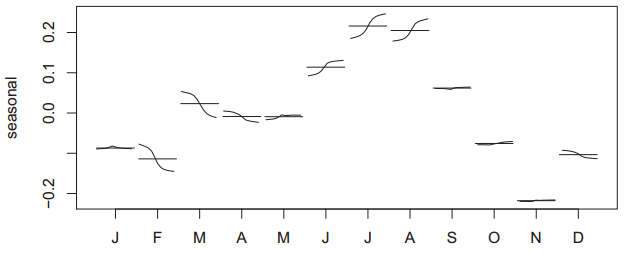
\includegraphics[width=1\linewidth]{images/tsMonthplot.png}
	\subcaption{Cycle-subseries of the STL decomposition}
	\label{Fig:tsMonthplot}
\end{minipage}
\end{figure}

}